% K字 例1：α=90°, PA=3, PB=4, AC=2 求 BD（示意图，按 K 字配置）
\documentclass[tikz,border=4pt]{standalone}
\usepackage{ctex}
\usepackage{amsmath}
\usetikzlibrary{calc}
\begin{document}
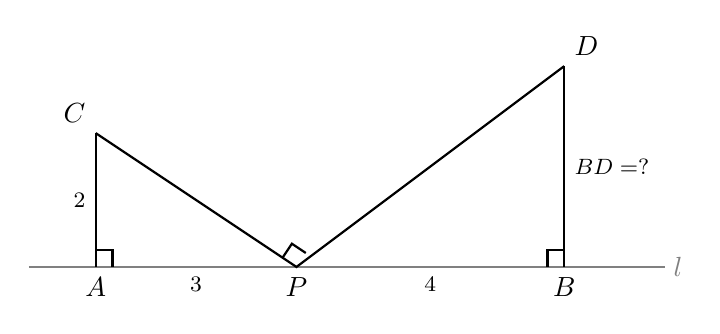
\begin{tikzpicture}[scale=0.85, thick]
  \draw[gray] (-4,0)--(5.5,0);
  \node[gray] at (5.7,0) {$l$};
  \coordinate (A) at (-3,0);
  \coordinate (P) at (0,0);
  \coordinate (B) at (4,0);
  \coordinate (C) at (-3,2);
  \coordinate (D) at (4,3);  % 示意位置
  \draw (A)--(C);
  \draw (C)--(P)--(D);
  \draw (B)--(D);
  % 三处直角
  \foreach \pt/\dx/\dy in {A/0.25/0, B/-0.25/0}{
    \draw ($(\pt)+(\dx,0)$) -- ($(\pt)+(\dx,0.25)$) -- ($(\pt)+(0,0.25)$);
  }
  % ∠CPD 直角 (P 处)
  \draw ($(P)+({0.25*cos(146.31)},{0.25*sin(146.31)})$)
        -- ($(P)+({0.25*cos(146.31)+0.25*cos(56.31)},{0.25*sin(146.31)+0.25*sin(56.31)})$)
        -- ($(P)+({0.25*cos(56.31)},{0.25*sin(56.31)})$);
  \node[below] at (A) {$A$};
  \node[below] at (P) {$P$};
  \node[below] at (B) {$B$};
  \node[above left] at (C) {$C$};
  \node[above right] at (D) {$D$};
  \node[left] at ($(A)!0.5!(C)$) {\footnotesize $2$};
  \node[below] at ($(A)!0.5!(P)$) {\footnotesize $3$};
  \node[below] at ($(P)!0.5!(B)$) {\footnotesize $4$};
  \node[right] at ($(B)!0.5!(D)$) {\footnotesize $BD=?$};
\end{tikzpicture}
\end{document}
